\chapter{Evaluating Siamese Neural Network Catalogue Matching Robustness}\label{ch:SNNEvaluation}

In this chapter the robustness of Siamese Neural Networks (SNNs) for the task of automatic most likely catalogue matching is explored. Beginning by examining the effects of NDD AU SMRU dataset variation on model performance, the generalisability of the approach is then examined through the use of a second photo-id catalogue. 

\section{Effect of AU SMRU Data on Model Performance}\label{ch:SNNEvaluation,sec:EffectOfAUSMRU}

As outlined in Section \ref{ch:NDD,sec:NDD_AU_SMRU}, additional photo-id data for 23 individuals were provided by the Universities of Aberdeen and St Andrews upon completion of fieldwork in the Coquet to St. Mary's Marine Conservation Zone. Whilst this data was primarily utilised to better understand the home range of resident cetaceans, it was also used to provide additional training data for automatic most likely catalogue matching, creating the NDD AU SMRU dataset and providing a larger number of class examples for initial SNN feasibility studies. 

Work undertaken throughout Chapter \ref{ch:ID} confirmed the ability of SNNs to perform most likely catalogue matching on the combined NDD AU SMRU dataset. To understand the effect of additional AU SMRU training data on model performance, two models were generated. First, a model was trained only on the data collected during the fieldwork season in Northumberland, UK. This data is contained within the Segmented NDD20 dataset discussed in Section \ref{ch:NDD,sec:postProcessingNDD20}. Due to the reduction in viable data for SNN training using semi-hard triplet mining, only 17 classes in Segmented NDD20 were utilised here in contrast to the 24 classes for model training on the full NDD AU SMRU dataset, discussed in Section \ref{ch:ID,sec:ModelSelection}. 

Next a second model was trained using the NDD AU SMRU dataset, limited to the 17 classes usable in Segmented NDD20. Evaluation of both models was performed using the 17 class NDD AU SMRU test set to allow for a like-for-like comparison. If both models perform equally well on the test set, it can be deduced that the inclusion of the AU SMRU data during training has not aided model generalisability. 

\begin{figure}
	\begin{center}
		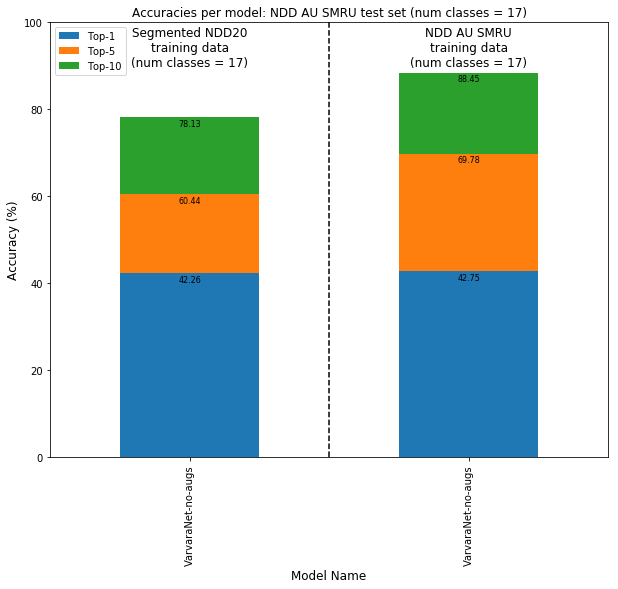
\includegraphics[scale=0.5]{Chapter6/figs/effect-of-au-smru.png}
	\end{center}
	\caption[Comparison between two SNNs trained for most likely catalogue matching, one using the Segmented NDD20 dataset, and the other using the NDD AU SMRU dataset.]{Comparison between two SNNs trained for most likely catalogue matching, one using the Segmented NDD20 dataset, and the other using the NDD AU SMRU dataset. Evaluation is performed using the NDD AU SMRU test set. All datasets limited to the 17 Segmented NDD20 classes suitable for SNN training with semi-hard triplet mining.}
	\label{fig:effect-of-au-smru}
\end{figure}

Figure \ref{fig:effect-of-au-smru} shows the top-1, top-5, and top-10 accuracies for both models when evaluated on the 17 class NDD AU SMRU test set. As can be seen, utilising the additional AU SMRU data as opposed to training solely on the Segmented NDD20 dataset provided a boost of 0.49\%, 9.34\%, and 10.30\% to top-1, top-5, and top-10 accuracies respectively. This supports the hypothesis that additional training examples improve most likely catalogue matching performance, even though the data was obtained from a secondary source. As such, this provides evidence to suggest that models trained on multiple photo-id catalogues may perform better than those trained on a single study, assuming there is some individual overlap.

However, performance of the model trained solely on the Segmented NDD20 dataset shows that even a model trained on the relatively small amount of data collected during the Northumberland fieldwork is able to greatly reduce the search space and can be utilised on data collected in a different spatio-temporal environment than the one on which it was trained, highlighting the robustness of the approach. 

\section{Effect of Background on Embedding Generation}\label{ch:SNNEvaluation,sec:EffectOfNoise}

Due to the free roaming nature of cetaceans, those in the NDD AU SMRU dataset were often photographed during only a single encounter leading to data with small intra-class but high inter-class background variation. This is similar to domains such as person re-identification, where images representing different classes often contain the same background information due to capture with a stationary camera. Recent work in this domain has shown that deep learning models may bias their similarity rankings based on background information \cite{tian_eliminating_2018}. 

To examine the effect that background removal has on downstream identification in the photo-id domain, an SNN was trained using the NDD AU SMRU dataset processed into bounding box class examples. All variables except the presence of background were kept consistent with those used when training the best performing mask SNN. Data for this experiment was generated using the same Mask R-CNN detector as for previous experiments, modified to output bounding boxes rather than masks. Corresponding dorsal fin masks for each bounding boxed image were taken from the NDD AU SMRU dataset, with background masks generated by inverting the fin mask. 

The bounding boxed fin, fin mask, and background mask were then embedded into the model's latent space, and the Euclidean distances between them calculated. This analysis showed that embedding generation is likely to be influenced more by features in the background than the fin. For example, the Euclidean distance between the bounding box data in Figure \ref{fig:bboxvsmask} (Left) and its corresponding dorsal fin mask (Centre) is 0.36, compared to a distance of 0.30 between the bounding box and the background mask (Right) and a mean distance of 0.97 between the bounding box and generated class prototypes. This suggests the SNN is performing likely matching based on features found in the background rather than on the dorsal fins, reflected in increased model performance whereby using bounding box data to train the SNN sees an increase of 22.94\% top-1, 15.58\% top-5, and 6.53\% top-10 accuracies over using masked data.

\begin{figure}
	\begin{center}
		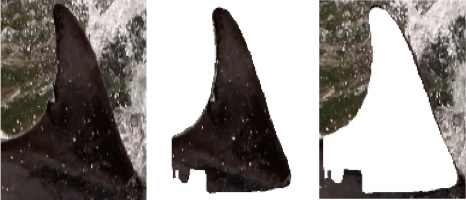
\includegraphics[scale=0.5]{Chapter6/figs/embedding-check-images.jpg}
	\end{center}
	\caption[Example data used to examine the effect of retained background on most likely catalogue matching.]{Example data used to examine the effect of retained background on most likely catalogue matching. Left: Bounding box detection containing both a dorsal fin and background. Centre: Corresponding dorsal fin mask. Right: Corresponding background mask.}
	\label{fig:bboxvsmask}
\end{figure}

By removing all background, the masked SNN is prevented from utilising environmental conditions to aid matching. This finding raises important questions regarding the performance of photo-id aids which do not remove all background before performing matching. Section \ref{ch:Background,sec:conTech,sub:photoIDAides,subsub:Summary} provides a summary of currently available photo-id aids. Of these, four works (Bouma \textit{et al.} \cite{bouma_individual_2018}, Lee \textit{et al.} \cite{lee_backbone_2020}, finFindR \cite{thompson_finfindr_2022}, and DolFin \cite{maglietta_dolfin_2018}) perform dorsal fin detection and downstream individual identification, however only Bouma \textit{et al.} and DolFin remove all background beforehand. If the photo-id catalogue utilised for evaluation of these systems has been collected over a small temporal scale, then results obtained in this experiment suggest that performance may be artificially inflated by the retention of feature heavy background. 

\section{Examining Siamese Neural Network Catalogue Matching Generalisability }\label{ch:SNNEvaluation,sec:SDRP}

As outlined in Chapter \ref{ch:ID}, an automatic approach to most likely catalogue matching was developed through the use of SNNs. This approach, when tested using the NDD AU SMRU dataset developed in Chapter \ref{ch:NDD}, yields high top-1, top-5, and top-10 accuracies. However, it is not yet clear if these results are to be expected regardless of the photo-id catalogue utilised, or if there is an underlying property inherent to the NDD AU SMRU dataset that makes it particularly susceptible to an SNN-based approach. In this chapter, automatic most likely matching is performed on a second, previously unseen, photo-id catalogue, allowing for an evaluation of the approach's generalisability.

\subsection{The SDRP Dataset}\label{ch:SNNEvaluation,sec:SDRP,sub:SDRPDataset}

To evaluate SNN generalisability, a subset of photo-id catalogue data was obtained from the Chicago Zoological Society's Sarasota Dolphin Research Program (SDRP)\nomenclature[z-SDRP]{SDRP}{Sarasota Dolphin Research Program}. The subset consisted of 250 images of 23 individual common bottlenose dolphins captured in the waters around Naples, FL, USA \cite{tyson_moore_final_2020}. Unlike the datasets collected from fieldwork in Northumberland, UK, the SDRP dataset was provided in a pre-processed form as the dataset had been previously utilised to compare photo-id methodologies \cite{tyson_moore_rise_2022}. Images provided were cropped to remove a large amount of background noise and centre the dorsal fin, examples of which can be seen in Figure \ref{fig:sdrp-example}. 

\begin{figure}
	\begin{center}
		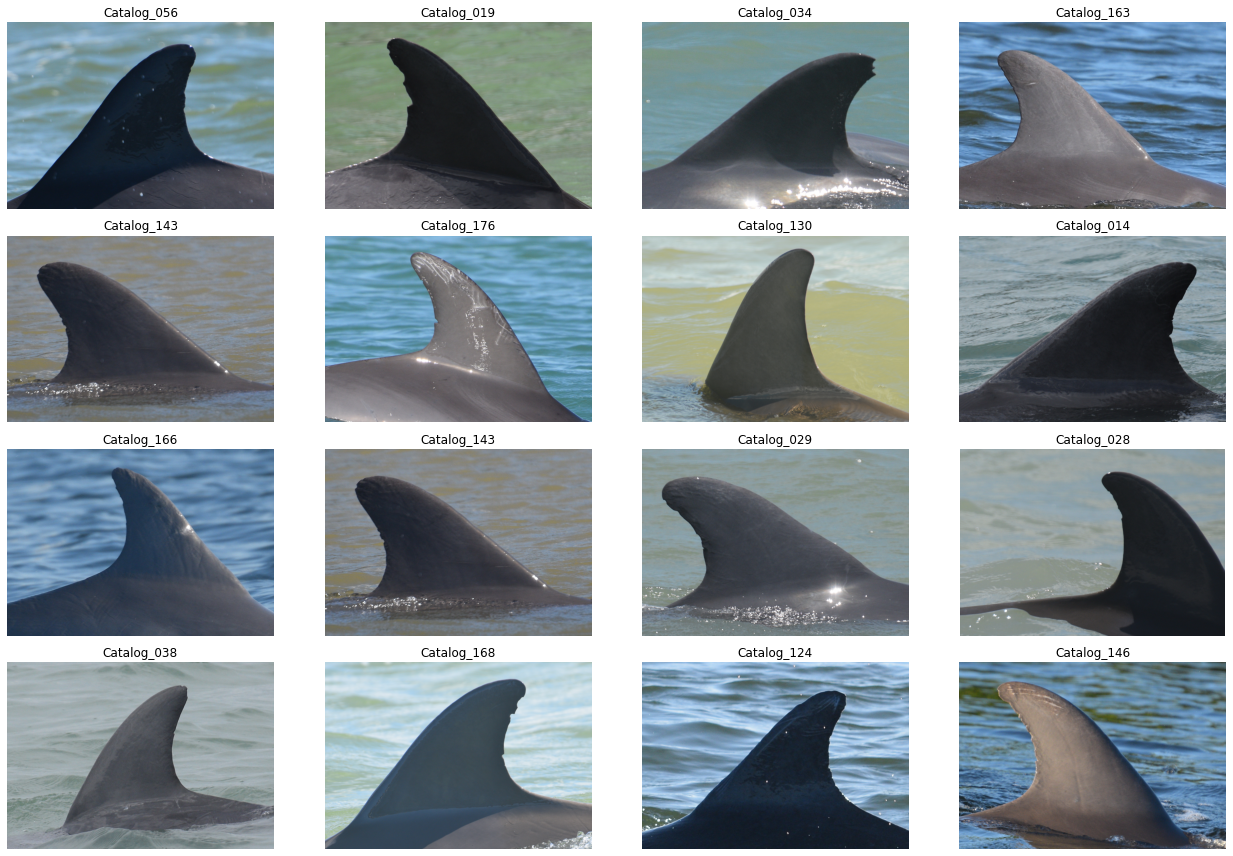
\includegraphics[scale=0.3]{Chapter6/figs/SDRP_egs_tiled.png}
	\end{center}
	\caption{Example images from the SDRP dataset with filenames displayed.}
	\label{fig:sdrp-example}
\end{figure}

The SDRP data was provided pre-split, with 200 images (each of a unique individual) acting as the existing photo-id catalogue, with the remaining 50 serving as images captured during a given day's fieldwork. Each image in the encounter set contained a single individual, however some individuals were captured multiple times. As such, there was a 23 individual overlap between the catalogue and encounter sets. 

To generate a train-test split capable of training an SNN, the catalogue set was reduced down to contain only the 23 individuals contained within the encounter set. Once filtered, both sets of images were run through the Mask R-CNN dorsal fin detector and post processed using morphological transformations, colour thresholding, and cropping -- outlined in Section \ref{ch:cetDet,sec:postProcessing}. No images in this dataset had been seen by the detector previously, either during training or evaluation. Once generated, a \texttt{noise} class was manually created which contained all erroneously detected mask components. However, as the detector failed to accurately detect examples of individual \texttt{19} this class was removed, resulting in a final dataset consisting of 23 classes. In cases where the detector had mistakenly detected the same fin twice, provided the two masks were not identical then both masks were kept -- analogous to offline data augmentation. An example of this can be seen in Figure \ref{fig:sdrp-double-mask-eg}.

\begin{figure}
	\begin{center}
		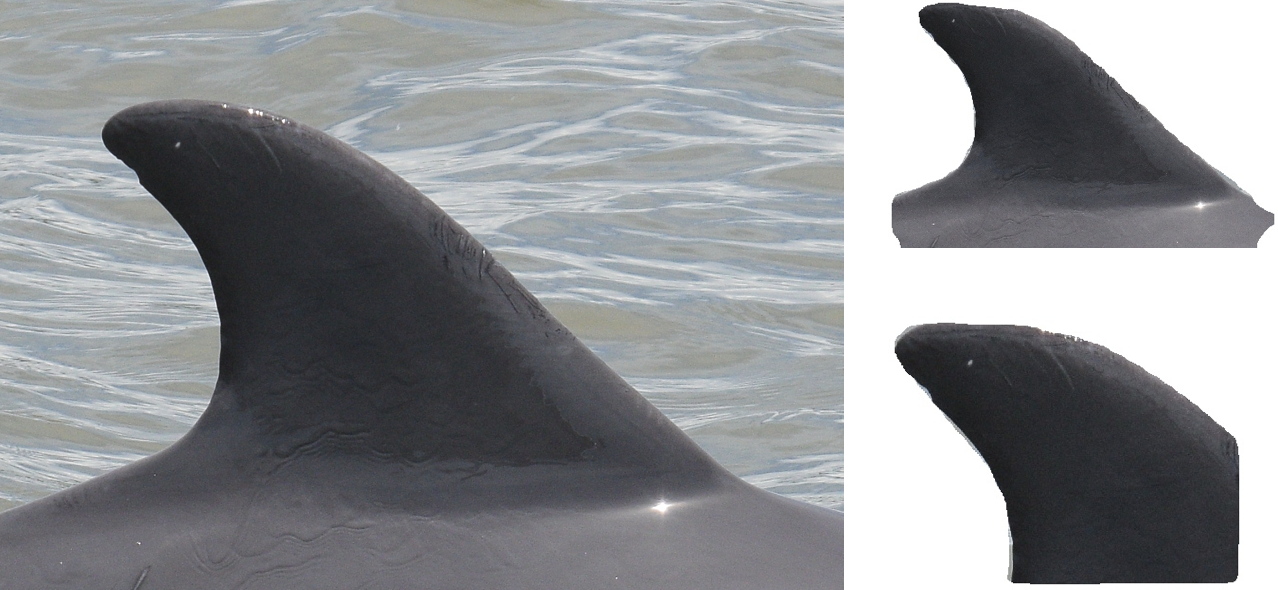
\includegraphics[scale=0.5]{Chapter6/figs/SDRP-double-mask-eg-indv-13.png}
	\end{center}
	\caption[Left: Image of individual \texttt{13} from the original SDRP catalogue set. Right: Example masks generated for the Left image.]{Left: Image of individual \texttt{13} from the original SDRP catalogue set. Right: Example masks generated for the Left image. Both masks are kept for use in training as they were deemed to be sufficiently different.}
	\label{fig:sdrp-double-mask-eg}
\end{figure}

After detection and processing the resultant SDRP dataset contained a total of 123 images, significantly smaller than the NDD AU SMRU dataset which was used to evaluate the SNN-based approach previously. Retaining the split provided by the SDRP, whereby the train set was generated from the catalogue and the test set from the encounter, leads to a 35-65 train-test split, an inversion of what would be expected when training machine learning models. The class distribution for the SDRP dataset can be seen in Figure \ref{fig:sdrp-dist}. As with the NDD AU SMRU dataset, the \texttt{noise} class is once again dominant. A colour threshold of 50\% was again utilised during post-processing with no correct detections erroneously discarded, suggesting this is an acceptable general value.

\begin{figure}[h]
	\begin{center}
		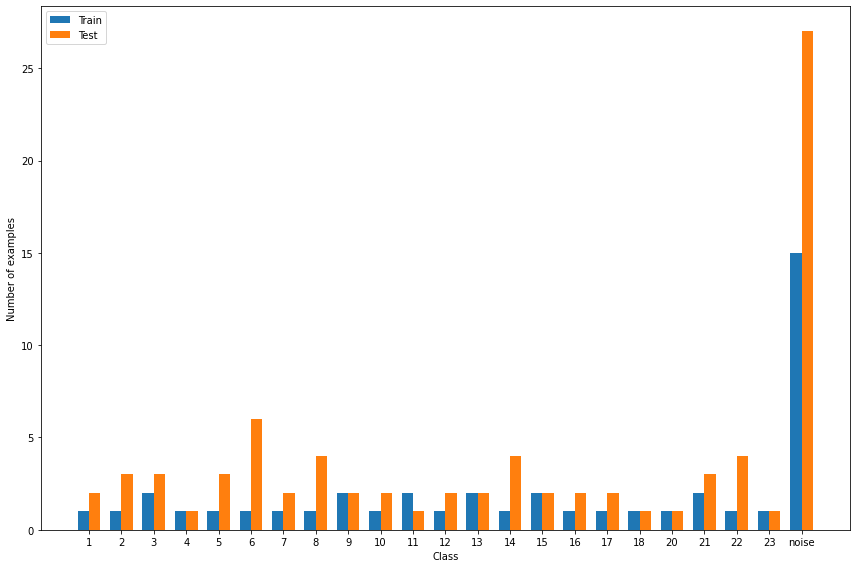
\includegraphics[scale=0.38]{Chapter6/figs/SDRP-class-dist.png}
	\end{center}
	\caption{The class distribution for the SDRP dataset, split by set.}
	\label{fig:sdrp-dist}
\end{figure}

These properties lead to the SDRP dataset being extremely challenging for an SNN to train on. However it is also an accurate representation of what a real life photo-id catalogue dataset would look like in the initial stages of a survey, providing an excellent test of both the robustness and generalisability of the SNN-based approach to automatic most likely catalogue matching when only small amounts of training data are available. 

\subsection{Evaluation Using the SDRP Dataset}\label{ch:SNNEvaluation,sec:SDRP,sub:SNNEvalWithSDRP}

Due to the small amount of data, it was not possible to create a meaningfully large and diverse validation set for the SDRP dataset. This prevented hyperparameter optimisation, and as such the decision was made to utilise the optimal hyperparameters located for the best performing SNN on the NDD AU SMRU dataset, alongside the same backbone architectures and data augmentation strategies defined in Section \ref{ch:ID,sec:SNNDevelopment}.

\begin{figure}[h]
	\begin{center}
		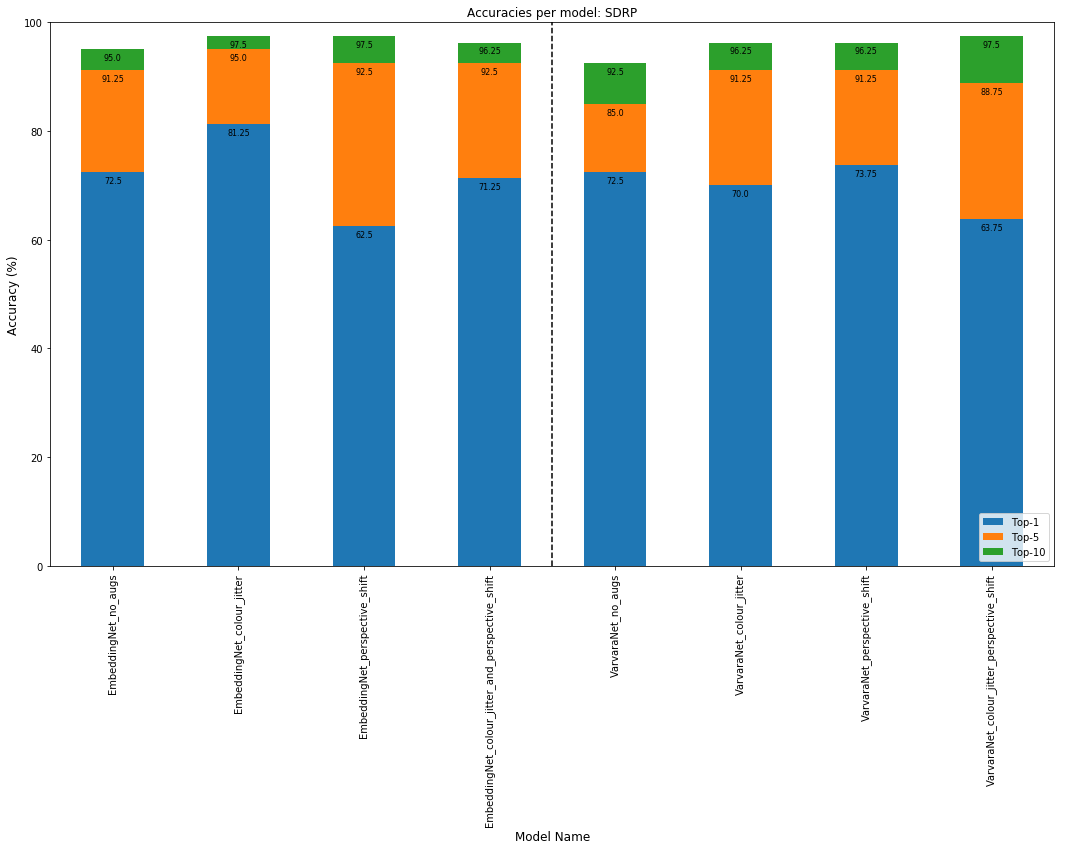
\includegraphics[scale=0.4]{Chapter6/figs/SDRP-normal-split-model-comparison.png}
	\end{center}
	\caption{Results of SNN training for the task of most likely catalogue matching on the SDRP dataset.}
	\label{fig:SDRP-normal-split-model-comparison}
\end{figure}

The results of model training on the SDRP dataset can be seen in Figure \ref{fig:SDRP-normal-split-model-comparison}, with each model evaluated using top-1, top-5, and top-10 accuracies.
Higher scores were achieved across the board on the SDRP dataset compared to the NDD AU SMRU dataset even without hyperparameter optimisation, however it is important to remember the smaller number of possible classes for the model to choose from which may inflate relative model performance.

Unlike the NDD AU SMRU data where best results were achieved without any augmentation, here the results are more mixed. Whilst the best top-10 accuracy, 97.50\%, is obtained using Colour Jitter and Perspective Shift augmentations (both together and separately), the best top-5 and top-1 accuracies were obtained using Colour Jitter only. These findings suggest that data augmentation strategy may be catalogue dependent and have a large impact on final model performance, and as such a search of possible data augmentation strategies should be performed each time an SNN model is trained using a new or updated photo-id catalogue. 

Variation in backbone architecture had little effect on overall model performance. Interestingly models trained using a VarvaraNet backbone were more consistent, with a 10.00\% difference between the best and worst performing model compared to an 18.75\% difference between those trained using an EmbeddingNet backbone. Overall however, the best performing model was determined to be an SNN using an EmbeddingNet backbone architecture and Colour Jitter data augmentation, which achieved 81.25\% top-1, 95.00\% top-5, and 97.50\% top-10 accuracies. This is in contrast to the best performing NDD AU SMRU model, made up of a VarvaraNet backbone architecture without any data augmentation. Using the optimal NDD AU SMRU model setup achieved 72.50\% top-1, 85.00\% top-5, and 92.50\% top-10 accuracies on the SDRP dataset. The use of an EmbeddingNet backbone as optimal for this dataset suggests that a simpler model structure may be best when working with smaller catalogues.

\subsection{SDRP Uncatalogued Individual Thresholding}\label{ch:SNNEvaluation,sec:SDRP,sub:uncatalogued}

Evaluation of the best performing SDRP model's ability to flag uncatalogued individuals was undertaken. Unlike the model trained on the NDD AU SMRU dataset, a write-up of which is provided in Section \ref{ch:ID,sec:ModelSelection}, when trained on the SDRP dataset embedded images are placed closer together in the latent space. This means that the threshold values utilised for uncatalogued individual detection using prototype distance measurement and K-Nearest Neighbours (KNN) required modification to accurately output the necessary warnings. 

Previous experimentation determined it was possible to flag potentially uncatalogued individuals by measuring the distance between an embedded image and its closest class prototype. For the NDD AU SMRU dataset, a minimum distance of 4.0 was required before a warning was displayed. Analysis of the distances between SDRP image embeddings and class prototypes however determined that this value was too large to be used with this latent space, as warnings were not displayed for some uncatalogued individuals when used. Through empirical examination of the distances between each image and the class prototypes, in agreement with the related literature \cite{battle_siamese_2022}, a threshold of 0.15 was determined to be optimal for the SDRP dataset, being small enough to trigger a warning for uncatalogued individuals whilst still being large enough not to trigger in error.

Alongside prototype distance measurement, KNN can also be utilised for uncatalogued individual warning generation. Rather than measuring distances between embeddings as with prototype thresholding, here warnings are generated by calculating an uncertainty score based on the class labels of the $K$ nearest embeddings. When processing the NDD AU SMRU dataset it was determined that setting $K$ to 10 was sufficient, producing a warning when no single class made up 30\% or less of the nearest class labels. 

For the SDRP dataset, whilst an uncertainty of 30\% was found to be sufficient for generating a warning, setting $K$ to 10 was deemed too high. Utilising this value resulted in some catalogued individuals incorrectly producing a warning as a result of the latent space's more compact nature. Evaluation of each test image's neighbours in the latent space determined that setting $K$ to 5 was optimal. Using this value ensured that warnings were displayed when uncatalogued individuals were processed, but prevented warning generation when processing examples of individuals present during training. 

\begin{figure}[t]
	\begin{center}
		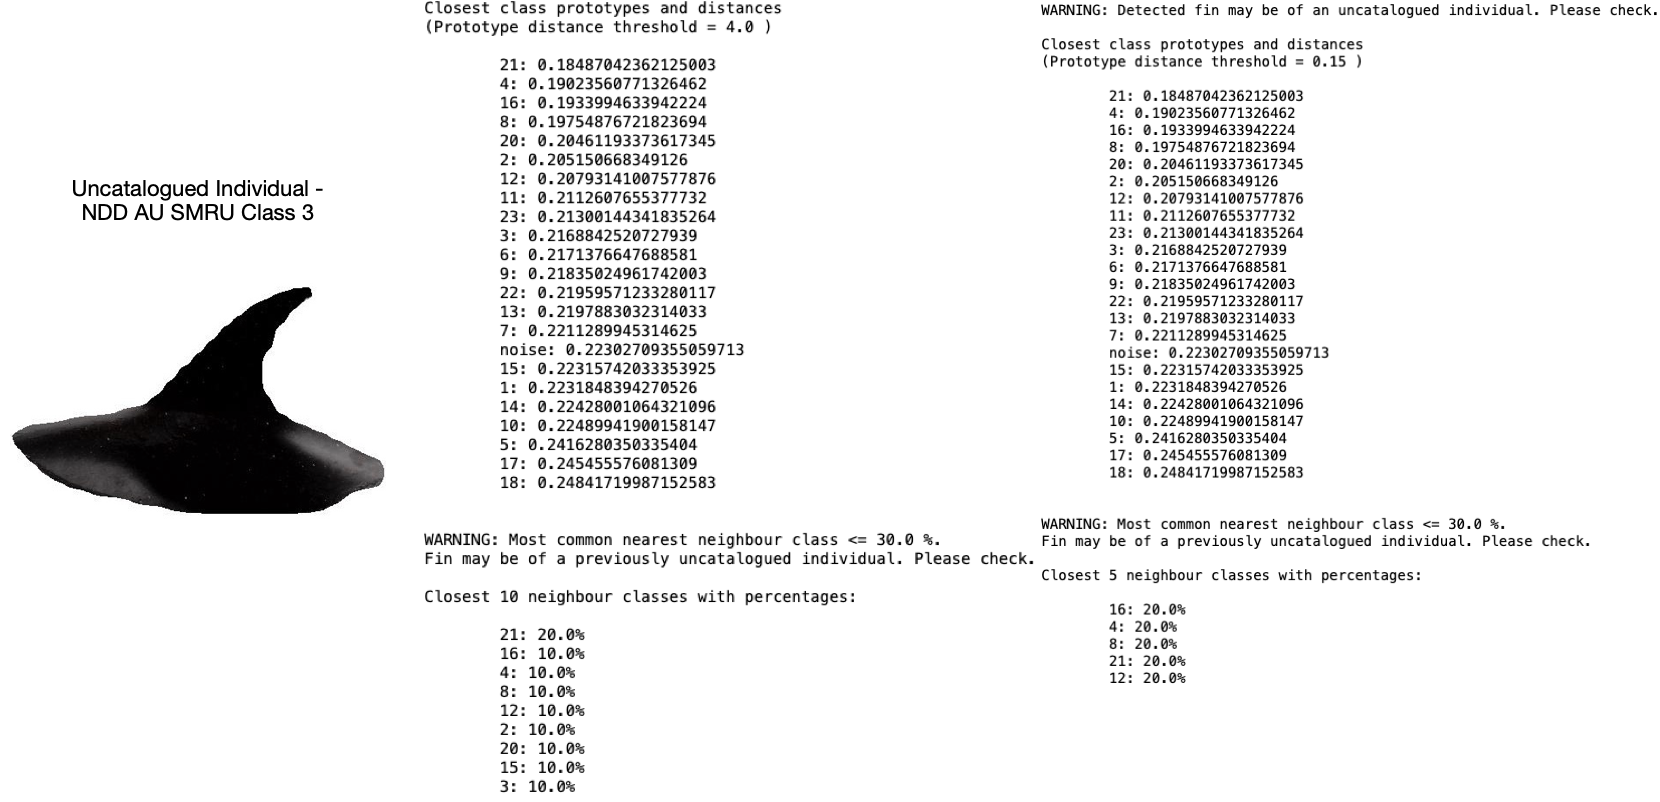
\includegraphics[scale=0.5]{Chapter6/figs/uncatalogued-individual-thresholding.png}
	\end{center}
	\caption[Example uncatalogued individual thresholding for the SDRP dataset using an individual not present during training.]{Example uncatalogued individual thresholding for the SDRP dataset using an individual not present during training (image taken from the NDD AU SMRU dataset). The resultant Euclidean distances between the input image's embedding and the existing class prototypes are shown. No warning has been generated when the minimum distance threshold is set to 4.0, however one has been when the threshold is set to 0.15. Uncertainty scores generated using K-Nearest Neighbours clustering are also shown. Warnings have been displayed both when $K = 10$ and $K = 5$ using an uncertainty threshold of $>=30\%$.}
	\label{fig:uncatalogued-individual-example-sdrp}
\end{figure}

Example warning generation using both prototype distance measurement and KNN for an uncatalogued individual can be seen in Figure \ref{fig:uncatalogued-individual-example-sdrp}. Here, an example from the NDD AU SMRU dataset has been processed by the SNN trained on the SDRP dataset, and so warnings should be generated both by prototype distance measurement and KNN. As can be seen, when utilising a minimum prototype distance of 4.0 no warning is generated. Changing this value to 0.15 however ensures a warning is generated. When checking using KNN, warnings are produced both when $K$ is set to 10 and 5. Figure \ref{fig:catalogued-individual-example-sdrp} shows example warning generation for an individual present during SNN training on the SDRP dataset. No warning has been generated with either minimum prototype distances, as expected. When $K$ is set to 10 however, a warning is erroneously generated. This is prevented by setting $K$ to 5. 

\begin{figure}
	\begin{center}
		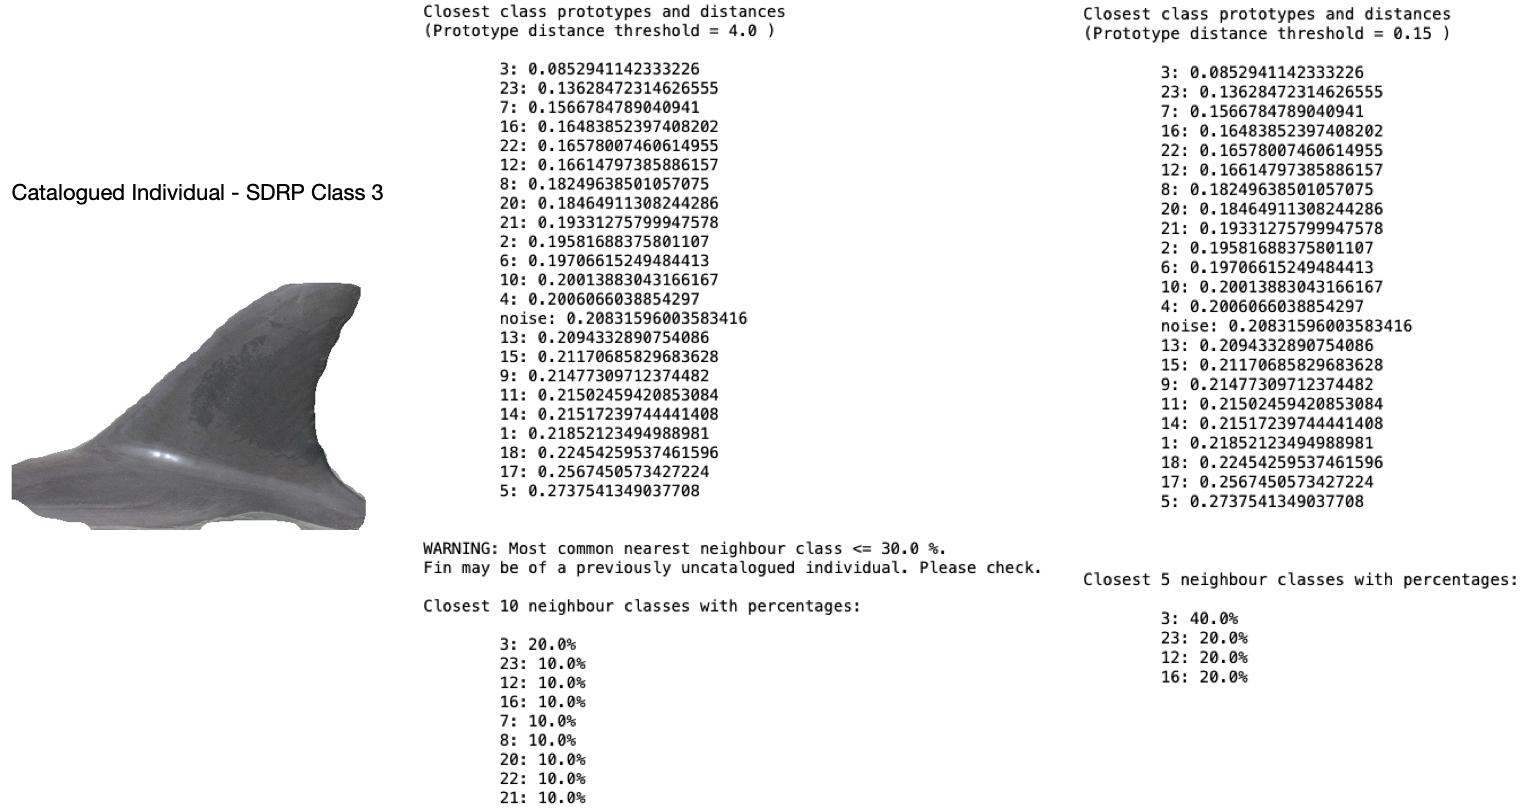
\includegraphics[scale=0.5]{Chapter6/figs/catalogued-individual-thresholding.png}
	\end{center}
	\caption[Example uncatalogued individual thresholding for the SDRP dataset using an individual present during training.]{Example uncatalogued individual thresholding for the SDRP dataset using an individual present during training. The resultant Euclidean distances between the input image's embedding and the existing class prototypes are shown. No warning has been generated when the minimum distance threshold is set to either 4.0 or 0.15. Uncertainty scores generated using K-Nearest Neighbours clustering are also shown. A warning is displayed when $K = 10$ but not when $K = 5$, with both using an uncertainty threshold of 30\%.}
	\label{fig:catalogued-individual-example-sdrp}
\end{figure}

Based on the experimentation described above, it can be seen that whilst uncatalogued individual detection can be performed on the SDRP catalogue using both prototype distance measurement and KNN as with the NDD AU SMRU catalogue, evidence suggests that threshold values for both techniques are catalogue dependent and require tuning before use. Whilst not tested here, it is thus likely that tuning is required if the model is retrained on an updated catalogue due to the change in data distribution. Further, whilst the KNN threshold values for flagging noise and uncatalogued individuals, $>=70\%$ and $<=30\%$  of an embedding's nearest neighbours respectively, were found to be sufficient for both catalogues examined in this work, there is no guarantee that this is the case for all catalogues globally. When adapting this work to a new catalogue, it is advised that consideration is given to all values used by both prototype distance measurement and KNN for the task of uncatalogued individual detection. It may be the case that this tuning can be automated by utilising the properties of the latent space to determine sufficient thresholds based on the training data, an approach which should be explored in future.

\subsection{Effect of Training Set Size on Model Backbone Selection}\label{ch:SNNEvaluation,sec:SDRP,sub:SDRPDataset,sub:reversedSDRP}

 As previously mentioned, the SDRP catalogue was provided pre-split which, once post-processed, produced a 35-65 train-test divide. As this training set is much smaller than what would normally be expected for developing a deep learning model, experimentation was undertaken to evaluate the hypothesis that a simpler model structure is best when low volumes of catalogue data are available during training. To this end, the dataset splits were reversed such that the test set was used for model training and the train set was used for evaluation. For consistency, the same model backbones and data augmentation strategies were utilised during training, as were the optimal NDD AU SMRU hyperparameters. 

 \begin{figure}[t]
 	\begin{center}
 		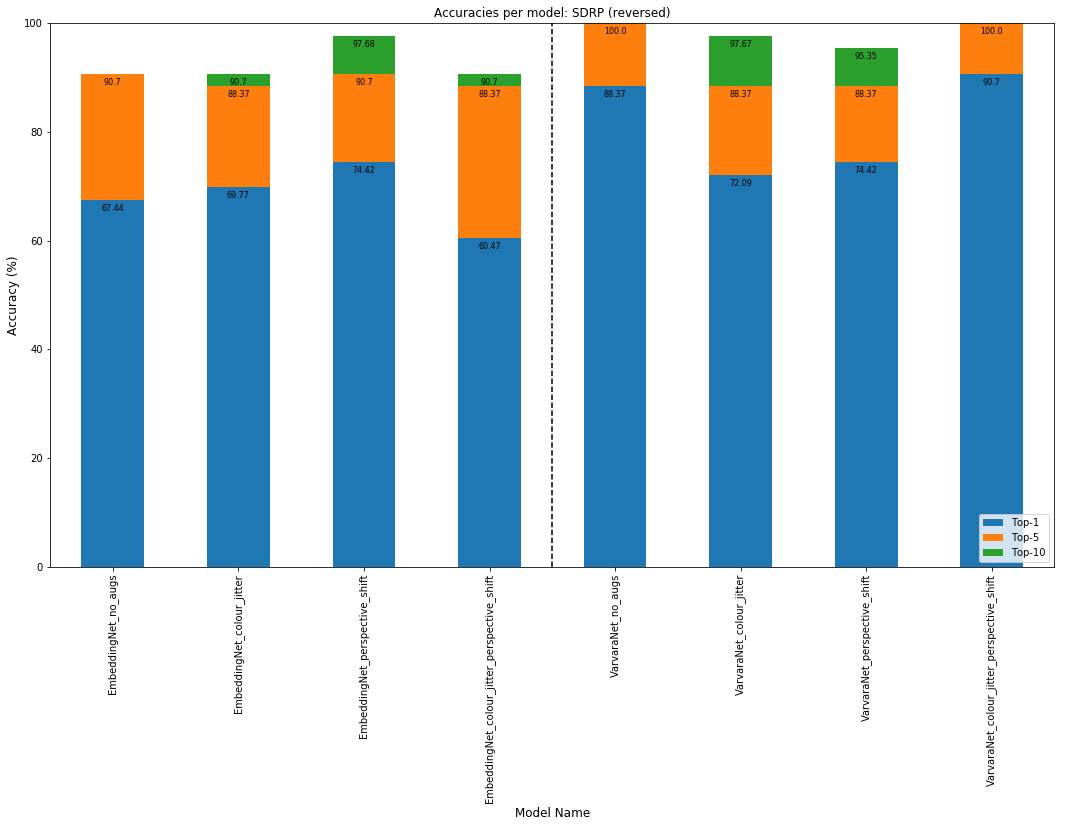
\includegraphics[scale=0.4]{Chapter6/figs/SDRP-reversed-split-model-comparison.png}
 	\end{center}
 	\caption{Results of SNN training for the task of most likely catalogue matching on the reversed SDRP dataset.}
 	\label{fig:SDRP-reversed-split-model-comparison}
 \end{figure}

The top-1, top-5, and top-10 accuracies for the trained models can be seen in Figure \ref{fig:SDRP-reversed-split-model-comparison}. By reversing the train-test split, a drop in performance is observed for all bar one of the models trained using an EmbeddingNet backbone. For the single model where performance improves, increases of 11.92\% top-1 and 0.18\%  top-10 accuracies are observed, however a drop of 1.80\% top-5 accuracy is also seen. For those models trained using a VarvaraNet backbone, increases in performance are observed for all models, with only two reporting slight drops in top-5 accuracy. 

In general, it can be observed that the increase in training data has led to an overall performance boost for models trained using a VarvaraNet backbone whilst those with an EmbeddingNet backbone observe a performance drop. As such, the best performing model for the reversed split SDRP dataset now makes use of a VarvaraNet backbone alongside both Colour Jitter and Perspective Shift data augmentation strategies. This supports the hypothesis that backbone architecture selection is influenced by the size of the initial training set, a finding backed up by other works in the area \cite{dutta_evaluation_2018, sug_effect_2010}. Further, it seems to be the case that more complex models are required to fully capture the fine-grained nature of larger photo-id catalogues. These findings also provide further evidence to support the idea that data augmentation strategies are catalogue dependent. 

It should be noted however that the best performing model achieves 100\% top-5 and top-10 accuracies, suggesting the possibility of model overfitting. Whilst the model may be capable of always providing a match within the first five results, this is likely a product of dataset size causing an inflation in model performance. It is expected that these accuracies would decrease when utilising more data, either through an increase in the number of classes or examples per class, as this would provide an increase in data variation.

\section{Considering Catalogue Matching as a Standard Classification Task}\label{ch:SNNEvaluation,sec:comparsion}

In order to better understand the performance of SNNs for the task of most likely catalogue matching, an evaluation was undertaken whereby the task was approached as a standard image classification problem. Using the NDD AU SMRU dataset, standard architectures (ResNet50, ResNet101 \cite{he_deep_2015}, and VGG16 \cite{simonyan_very_2015}) were trained and evaluated against top-1, top-5, and top-10 accuracy metrics. This range was chosen to help identify whether model depth or setup has an effect on classification performance. 

As these models only require a single example image per training step, rather than a triplet of images as required when training SNNs with Triplet Ranking Loss, Cross Entropy Loss was instead utilised. This function compares the predicted class probabilities outputted by the model to those of the ground truths (either $0$ or $1$ in this case). A loss is computed using Equation \ref{eq:crossEntropyLoss} (where $n$ is the number of classes, $t$ is the ground truth label probability, and $p$ is the Softmax probability for the $i^{th}$ class) which in turn can be used to inform how the weights of the model should be changed. A model which performs perfectly would yield a Cross Entropy Loss of 0. 

\begin{equation}
	\label{eq:crossEntropyLoss}
	L = -\sum_{i=1}^{n} t_{i} log(p_{i})
\end{equation}

Bayesian hyperparameter optimisation during model training was performed using the Optuna framework \cite{akiba_optuna_2019}, as in Section \ref{ch:ID,sec:SNNDevelopment,sub:Optuna}. Due to the required change in loss function, the total number of hyperparameters required by the models was reduced. The search aimed to find an optimal \texttt{log uniform} learning rate between $1\times10^{-6}$ and $1\times10^{-3}$, a dropout \cite{srivastava_dropout:_2014} \texttt{uniform} probability between 0.1 and 0.7, a \texttt{log uniform} weight decay between $1\times10^{-6}$ and $1\times10^{-1}$, an \texttt{int} step size between 5 and 10, and a $\gamma$ \texttt{log uniform} value between $1\times10^{-3}$ and $1\times10^{-1}$. The learning rate optimiser was also tuned, allowing for a \texttt{categorical} choice between SGD or Adam \cite{kingma_adam:_2014}, as well as whether the model started from a pre-trained state or not, with ImageNet \cite{krizhevsky_learning_2009} weights utilised if pre-training was required. A total of 100 iterations were undertaken, with the optimal hyperparameters for each final model architecture decided by its best performing trial. The optimal hyperparameters for each model architecture can be seen in Appendix \ref{app:standard}. To fit the models into memory, the number of samples per class for each training batch was reduced from 9 when training SNNs to 3 for ResNet50, and 2 for ResNet101 and VGG16.

The top-1, top-5, and top-10 accuracies for the best performing models can be seen in Table \ref{tab:optunaBestParamsStandard}. Compared to the best performing SNN, these models all struggle to accurately classify the individuals present in the NDD AU SMRU dataset, with ResNet101 performing best. This lack of accuracy is hypothesised to be due to the extreme fine-grained nature and high intra-class variability of the dataset. For comparison, the best performing SNN trained on this dataset achieves 36.78\%, 54.47\%, and 55.28\% higher top-1, top-5, and top-10 accuracies respectively. 

\begin{table}[]
	\centering
	\small
		\begin{tabular}{cccc}
			\cline{2-4}
			 & \multicolumn{3}{c}{\textbf{Accuracy (\%)}} \\ \hline
			\textbf{Architecture}                    &  \textbf{Top-1} & \textbf{Top-5} & \textbf{Top-10} \\ \hline
			ResNet50 \cite{he_deep_2015}   &  3.46                 & 11.79            & 27.03                  \\
			ResNet101 \cite{he_deep_2015}   &  4.07                  &   14.43               &  27.85                     \\
			VGG16 \cite{simonyan_very_2015} & 2.64                &    15.45              &   33.54     \\\bottomrule
	\end{tabular}
	\caption[Top-$N$ accuracies of the best performing image classification models on the NDD AU SMRU dataset.]{Top-$N$ accuracies of the best performing image classification models on the NDD AU SMRU dataset. Accuracies given to 2 decimal places.}
	\label{tab:optunaBestParamsStandard}
\end{table}

Examining the Bayesian optimised hyperparameter tuning runs suggests that starting from a pre-trained state is the most important indicator of model performance when utilising a ResNet architecture for this task. An example of this can be seen in Figure \ref{fig:resnet50baseline-hyperparam-importance-optuna} which shows the hyperparameter importances for the ResNet50 tuning run, including a pre-training importance of 0.81 -- for ResNet101 this value was 0.72. Whilst it is expected that this hyperparameter would have high importance due to the relatively small size of the NDD AU SMRU dataset and deepness of the architectures, the lack of importance for all other hyperparameters may suggest that this model setup is incapable of identifying meaningful features which allow the models to consistently differentiate between classes. 

\begin{figure}
	\begin{center}
		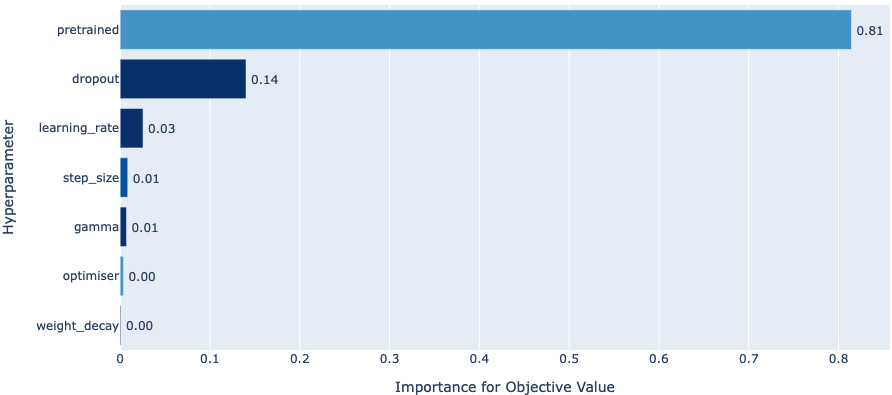
\includegraphics[scale=0.4]{Chapter6/figs/resnet50baseline-hyperparam-importance-optuna.png}
	\end{center}
	\caption{Importance scores for the hyperparameter tuning of the ResNet50 model.}
	\label{fig:resnet50baseline-hyperparam-importance-optuna}
\end{figure}

When training the VGG16 model however, the optimal model found did not require pre-training, with a hyperparameter importance of 0.02. Instead, weight decay was the most important hyperparameter with an importance of 0.39 as seen in Figure \ref{fig:vgg16baseline-hyperparam-importance-optuna}. This lack of pre-training importance may be due to the shallower depth of the architecture. However, as seen in Table \ref{tab:optunaBestParamsStandard}, the VGG model also did not achieve high accuracies on the NDD AU SMRU dataset. 

\begin{figure}
	\begin{center}
		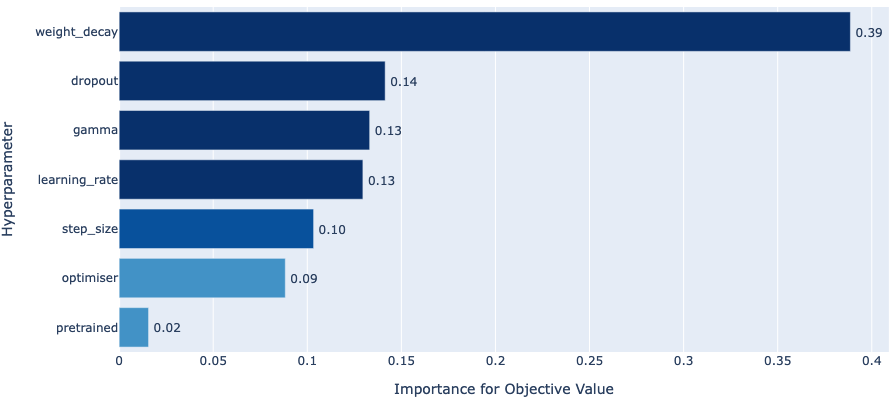
\includegraphics[scale=0.4]{Chapter6/figs/vgg16-baseline-hyperparam-importance-optuna.png}
	\end{center}
	\caption{Importance scores for the hyperparameter tuning of the VGG16 model.}
	\label{fig:vgg16baseline-hyperparam-importance-optuna}
\end{figure}

These findings suggest that the use of triplets when training SNNs may allow for more meaningful features to be extracted, leading to more accurate most likely catalogue matching. As such, this indicates that the use of an SNN to generate embeddings, plotting these into a latent space, and utilising clusters to provide most likely matches is a superior approach to training a standard image classifier, notwithstanding the difficulties which would arise if individuals not seen at train time were required to be classified.

\section{Summary}\label{ch:SNNEvaluation,sec:Summary}

This chapter examines the robustness of SNNs for the task of automatic most likely catalogue matching. To begin, the effect on model performance of additional photo-id data is examined. This work shows that while the additional data improves overall generalisability, a model capable of vastly reducing the search space can be obtained utilising only the data collected in a single fieldwork study, even when running inference on data from a different spatio-temporal environment.

Next, the effect of background retention on embedding generation is examined. By training a model using bounding box imagery rather than masks and examining the embeddings generated for various inputs, it can be seen that embeddings can be influenced more by feature heavy background surrounding a dorsal fin than the fin itself, at least when the model is trained on data collected over a small spatio-temporal scale. This emphasises the importance of detection masks over bounding boxes, further reinforcing the decision made in Section \ref{ch:cetDet,sec:deciding,sub:boundingBoxInvestigation}.

The generalisability of utilising SNNs for the task of automatic most likely catalogue matching is then examined through the use of a second smaller photo-id catalogue provided by the Chicago Zoological Society's Sarasota Dolphin Research Program. Training an SNN on this data yields a model which is highly accurate, achieving 81.25\% top-1, 95.00\% top-5, and 97.50\% top-10 accuracies. This provides evidence to suggest that SNNs are a viable approach to automatic most likely matching, regardless of catalogue size, species, or environment.

Finally, the task of most likely catalogue matching is framed as a standard image classification problem in order to provide a baseline with which to compare the previously developed SNN approach. Experiments show that the standard model architectures trained, ResNet50, ResNet101, and VGG16, are incapable of classifying images in the NDD AU SMRU dataset with high accuracy. This is hypothesised to be a result of the extreme fine-grained nature and high intra-class variability rendering the models incapable of identifying meaningful features for classification, which could be negated thanks to the use of triplets during training and clustering generated embeddings into a latent space.

Experimentation throughout this chapter has shown that SNNs are an accurate and generalisable approach to the task of catalogue matching. When accompanied by a dorsal fin detector and post-processing methodology, a fully automatic photo-id aid can be created which is robust to changes in species of interest, geography, and time. A summary of the work undertaken throughout this thesis to develop an automatic photo-id aid is provided in Chapter \ref{ch:Conclusion}. Possible avenues for further work are also explored in detail.
